
\section{Introduction}
\label{sec:introduction}

This document describes the installation process and the first steps
of using the Eclipse Coordination Tools (ECT) for developing
component-based software. In this section, we give a short introduction Reo---a
channel-based coordination language which is specification language for
modeling component connectors in our tools.

\subsection{Reo Overview}
\label{sec:reo-overview}

Reo is a channel-based coordination language wherein channels are primitive,
user-defined entities that have two ends which can be either \emph{sources} or
\emph{sinks}. Source ends accept data into and sink ends dispense
data out of channels.
%
% Explaining the basic channel types:
%
Each channel type imposes its own constraints on the possible data flow at its
ends, e.g. synchrony or mutual exclusion. For instance, the \Sync channel
(\sync) synchronously reads data items from its source end and writes it to its
sink end without buffering them. The \LossySync (\lossysync) behaves
similarly, except that it looses the data when no one is ready
to read it from its sink end. While these two channels are both unbuffered, the
\FIFO (\fifo) can store a single data item and release it again when someone
tries to read from it. The \SyncDrain (\syncdrain) has--unlike the channels
introduced so far--two source ends and hence is not directed. If there are data items
available at each of its ends, this channel consumes both of them synchronously.

% How to build connectors from channels and nodes:

Channels can be composed by joining them into nodes. Such a composite structure
is called a \emph{connector} in Reo and has some similarities with electrical
circuits. As mentioned before, channels are user-defined. However, nodes have 
a fixed behaviour in Reo. A node atomically does a destructive read at one
of the sink ends and replicates the data item at all of its attached source ends.
With this simple behaviour of nodes and a small set of basic channels, complex
protocols can be implemented compositionally, i.e. by just plugging together
channels and nodes.

% Examples:
\begin{figure}[ht]
	\begin{center}
	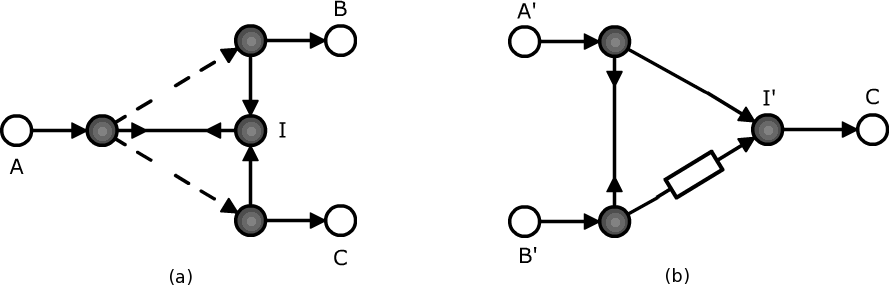
\includegraphics[height=4cm]{images/router-ordering}
	\end{center}
\caption{a) \emph{exclusive router}, b) \emph{ordering} connector.}
\label{fig:router-ordering}
\end{figure}

For instance, the \emph{exclusive router}, shown in
Fig.~\ref{fig:router-ordering}a, routes data from $A$ to either $B$ or $C$.
If both, $B$ and $C$, are able to receive data the choice is made
nondeterministically. The mutual exclusion that is implemented by this connector
is due to the fact that the internal node $I$ allows input only from exactly
one of its sink ends. The second connector, shown in Figure
\ref{fig:router-ordering}b, imposes an ordering on the data flow from the
input nodes $A'$ and $B'$ to the output node $C'$. The \SyncDrain synchronises
the two inputs and the \FIFO delays the items from $B'$.

The minimalistic set of core concepts that Reo introduces is surprisingly
powerful. A number of formalisms have been invented to model the
different facets of Reo connectors (see, e.g., \cite{ABRS03,AR02,CCA05}). 
These formalisms are not only nice from the theoretical point of
view, but they further serve as a strong basis for implementing
Reo. This includes tools for the modeling and verification of connectors 
(i.e. interaction protocols) as well as actual runtime engines.


\subsection{Constraint Automata}
\label{sec:constraint-automata}

\subsection{Coloring Semantics}
\label{sec:coloring-semantics}

